% Compile with XeLaTeX (Overleaf: Menu -> Compiler -> XeLaTeX)
\documentclass[12pt,a4paper]{extreport}
\usepackage{fontspec}
\usepackage{polyglossia}

% ---- Տառատեսակ. նմուշի պես GHEA Grapalat, եթե հասանելի է; հակառակ դեպքում DejaVu Serif ----
% Overleaf-ում. GHEAGrapalat.ttf ֆայլը վերբեռնել thesis/fonts/ պանակ
\IfFontExistsTF{GHEA Grapalat}{%
  \setmainfont{GHEA Grapalat}
  \newfontfamily\armenianfont{GHEA Grapalat}
}{%
  \IfFileExists{fonts/GHEAGrapalat.ttf}{%
    \setmainfont{GHEAGrapalat.ttf}[Path=fonts/,AutoFakeBold=3]
    \newfontfamily\armenianfont{GHEAGrapalat.ttf}[Path=fonts/,AutoFakeBold=3]
  }{%
    \setmainfont{DejaVu Serif}
    \newfontfamily\armenianfont{DejaVu Serif}
  }%
}
\setmonofont{DejaVu Sans Mono}
\newfontfamily\armenianfonttt{DejaVu Sans Mono}
\setmainlanguage[numerals=arabic]{armenian}
\setotherlanguage{english}

\usepackage{amsmath,amssymb,amsthm}
\usepackage{array}
\usepackage{graphicx}
\usepackage[hidelinks]{hyperref}
% ---- Էջի ձևաչափ (ըստ նմուշի). A4, ձախ 3 սմ, աջ 1 սմ, վերև 2 սմ, ներքև 2,5 սմ ----
\usepackage[a4paper,left=3cm,right=1cm,top=2cm,bottom=2.5cm]{geometry}
\usepackage{microtype}
\usepackage{setspace}
\usepackage{indentfirst}
\usepackage{fancyhdr}
\usepackage{titlesec}
\emergencystretch=4em
\sloppy
\onehalfspacing                 % 1,5 ինտերվալ
\setlength{\parindent}{1.25cm}  % պարբերության ներքաշում
\setlength{\parskip}{0pt}

% էջի համարը՝ ներքևում աջ կողմում
\pagestyle{fancy}\fancyhf{}\fancyfoot[R]{\thepage}\renewcommand{\headrulewidth}{0pt}
\fancypagestyle{plain}{\fancyhf{}\fancyfoot[R]{\thepage}\renewcommand{\headrulewidth}{0pt}}

% վերնագրեր. գլուխ՝ 16pt թավ, կենտրոնում, մեծատառ (վերնագրերը գրվում են մեծատառով)
\titleformat{\chapter}[block]{\centering\bfseries\fontsize{16}{20}\selectfont}{ԳԼՈՒԽ~\thechapter.}{0.5em}{}
\titleformat{name=\chapter,numberless}[block]{\centering\bfseries\fontsize{16}{20}\selectfont}{}{0pt}{}
\titlespacing*{\chapter}{0pt}{0pt}{18pt}
\titleformat{\section}{\bfseries\fontsize{14}{18}\selectfont}{\thesection.}{0.5em}{}
\titleformat{\subsection}{\bfseries\fontsize{12}{16}\selectfont}{\thesubsection.}{0.5em}{}
\addto\captionsarmenian{\renewcommand{\bibname}{Գրականության ցանկ}}

\newtheorem{theorem}{Թեորեմ}
\newtheorem{definition}{Սահմանում}
\newtheorem{example}{Օրինակ}

\begin{document}

\thispagestyle{empty}
\begin{center}
% TODO: ավելացնել համալսարանի, ֆակուլտետի և ամբիոնի անվանումը՝ ըստ ձեր ֆակուլտետի պահանջի
\vspace*{3cm}
{\large Դիպլոմային աշխատանք}\\[1.2cm]
{\Large\bfseries Գրաֆների կապակցվածության և ցանցի հուսալիության\\վերլուծության մեթոդների ուսումնասիրություն}\\[2cm]
\begin{flushright}
Կատարող՝ Ս.~Համբարձումյան\\[0.4cm]
Ղեկավար՝ Ն.~Բադալյան
\end{flushright}
\end{center}
\vfill
\begin{center}Երևան 2026\end{center}
\clearpage

\tableofcontents
\clearpage

% Ներածություն (սևագիր v1)

\chapter*{Ներածություն}
\addcontentsline{toc}{chapter}{Ներածություն}

Ժամանակակից հաղորդակցական, համակարգչային, էներգետիկ և տրանսպորտային ցանցերը հնարավոր է մոդելավորել գրաֆներով, որտեղ գագաթները ցանցի հանգույցներն են, իսկ կողերը՝ նրանց միջև կապերը: Ցանցի հիմնական պահանջներից մեկը կապակցվածությունն է. հանգույցների միջև պետք է պահպանվի կապ նույնիսկ առանձին տարրերի խափանման դեպքում:

\textbf{Թեմայի արդիականությունը.} Ցանցերի աճող բարդության և կարևորության պատճառով անհրաժեշտ է ունենալ մեթոդներ, որոնք թույլ են տալիս քանակապես գնահատել ցանցի կայունությունը խափանումների նկատմամբ: Գրաֆների տեսությունը տալիս է կառուցվածքային չափանիշներ (կտրող կետեր, կամուրջներ, $k$-կապակցվածություն), իսկ հուսալիության տեսությունը՝ հավանականային գնահատականներ: Այդ երկու մոտեցումների համատեղ ուսումնասիրությունը թույլ է տալիս ոչ միայն գտնել ցանցի խոցելի տեղերը, այլև համեմատել տարբեր կառուցվածքները:

\textbf{Աշխատանքի նպատակը} գրաֆների կապակցվածության և ցանցի հուսալիության վերլուծության հիմնական մեթոդների ուսումնասիրությունն է, դրանց համեմատությունը և կիրառումը կոնկրետ ցանցերի վրա:

\textbf{Խնդիրները.}
\begin{enumerate}
  \item ներկայացնել գրաֆների կապակցվածության հիմնական հասկացությունները և թեորեմները.
  \item դիտարկել կապակցվածության որոշման և չափման ալգորիթմները.
  \item ներկայացնել ցանցի հուսալիության մոդելները և հաշվարկի մեթոդները (ճշգրիտ հաշվարկ, Monte Carlo սիմուլյացիա).
  \item համեմատել մեթոդները ըստ ճշգրտության և հաշվողական բարդության.
  \item իրականացնել ծրագրային մոդել և փորձարկել այն օրինակելի ցանցերի վրա:
\end{enumerate}

\textbf{Աշխատանքի կառուցվածքը.} Աշխատանքը բաղկացած է ներածությունից, երեք գլխից, եզրակացությունից և գրականության ցանկից: Առաջին գլխում ներկայացվում են տեսական հիմքերը, երկրորդում՝ մեթոդները, երրորդում՝ գործնական մասը:


% Գլուխ 1. Տեսական հիմքեր (սևագիր v1)

\chapter{Տեսական հիմքեր}

\section{Գրաֆների հիմնական հասկացություններ}

\begin{definition}
\emph{Պարզ չուղղորդված գրաֆ} $G=(V,E)$ անվանում են զույգ, որտեղ $V$-ն վերջավոր բազմություն է (\emph{գագաթներ}), իսկ $E$-ն $V$-ի երկտարր ենթաբազմությունների բազմություն է (\emph{կողեր}): Նշանակենք $n=|V|$, $m=|E|$:
\end{definition}

Գագաթի $v$ \emph{աստիճան} $\deg(v)$ կոչվում է նրան կից կողերի թիվը: Գրաֆի նվազագույն աստիճանը նշանակենք $\delta(G)$:

\begin{definition}
\emph{Ուղի} է կոչվում գագաթների $v_0,v_1,\dots,v_k$ հաջորդականությունը, որտեղ ամեն $\{v_{i-1},v_i\}$ կող է և գագաթները զույգ առ զույգ տարբեր են: \emph{Ցիկլ} է կոչվում փակ ուղին (երբ $k\ge 3$ և $v_k=v_0$, մնացած գագաթները տարբեր են):
\end{definition}

\begin{definition}
Գրաֆը \emph{կապակցված} է, եթե նրա ցանկացած երկու գագաթների միջև գոյություն ունի ուղի: Գրաֆի \emph{կապակցվածության բաղադրիչը} նրա մաքսիմալ կապակցված ենթագրաֆն է:
\end{definition}

Գրաֆը կապակցված է այն և միայն այն դեպքում, երբ ունի ուղիղ մեկ կապակցվածության բաղադրիչ: Բաղադրիչները կարելի է գտնել BFS կամ DFS ալգորիթմով $O(n+m)$ ժամանակում (տե՛ս Գլուխ 2):

\begin{example}
Ցիկլը $C_n$ կապակցված է: Եթե նրանից հեռացնենք ցանկացած մեկ կող, կստացվի ուղի, որը դեռ կապակցված է: Եթե հեռացնենք ցանկացած երկու կող, գրաֆը կտրոհվի ուղիղ երկու կապակցվածության բաղադրիչի:
\end{example}

\section{Կապակցվածություն, կտրող կետեր, կամուրջներ}

\begin{definition}
Կապակցված գրաֆի $v$ գագաթը կոչվում է \emph{կտրող կետ}, եթե $G-v$ գրաֆը (գագաթը և նրան կից կողերը հեռացնելուց հետո) կապակցված չէ: Կապակցված գրաֆի $e$ կողը կոչվում է \emph{կամուրջ}, եթե $G-e$ գրաֆը կապակցված չէ:
\end{definition}

Ցանցային տերմիններով կտրող կետը \emph{միակ խոցելի հանգույցն} է, իսկ կամուրջը՝ \emph{միակ խոցելի կապը}, որի խափանումը բաժանում է ցանցը մասերի:

\begin{theorem}\label{thm:bridge}
Կապակցված $G$ գրաֆի $e=\{u,v\}$ կողը կամուրջ է այն և միայն այն դեպքում, երբ $e$-ն չի պատկանում ոչ մի ցիկլի:
\end{theorem}

\begin{proof}
Ենթադրենք $e$-ն պատկանում է ինչ-որ ցիկլի $C$: Այդ դեպքում $G-e$ գրաֆում $u$-ից $v$ ուղի կա՝ ցիկլի մնացած մասը: Ցանկացած ուղի, որն անցնում էր $e$-ով, կարելի է շրջանցել այդ ուղիով, ուստի $G-e$-ն կապակցված է, և $e$-ն կամուրջ չէ:

Հակառակը, ենթադրենք $e$-ն ոչ մի ցիկլում չի գտնվում, բայց $G-e$ կապակցված է: Այդ դեպքում $G-e$-ում կա $u$-ից $v$ ուղի $P$, և $P$-ն $e$-ի հետ կազմում է ցիկլ, որը պարունակում է $e$: Սա հակասում է ենթադրությանը, ուստի $G-e$ կապակցված չէ, այսինքն՝ $e$-ն կամուրջ է:
\end{proof}


\section{\texorpdfstring{$k$}{k}-կապակցվածություն և Մենգերի թեորեմը}

\begin{definition}
$G$ գրաֆի \emph{գագաթային կապակցվածություն} $\kappa(G)$ կոչվում է գագաթների նվազագույն թիվը, որոնց հեռացումը գրաֆը դարձնում է ոչ կապակցված կամ մեկ գագաթանի (լրիվ գրաֆի համար $\kappa(K_n)=n-1$): \emph{Կողային կապակցվածություն} $\lambda(G)$ կոչվում է կողերի նվազագույն թիվը, որոնց հեռացումը գրաֆը դարձնում է ոչ կապակցված: Գրաֆը \emph{$k$-կապակցված} է (կողային $k$-կապակցված), եթե $\kappa(G)\ge k$ (համապատասխանաբար $\lambda(G)\ge k$):
\end{definition}

\begin{theorem}[Ուիթնի անհավասարություն]
Ցանկացած գրաֆի համար $\kappa(G)\le\lambda(G)\le\delta(G)$:
\end{theorem}

Թեորեմի ապացույցը տե՛ս \cite{west}: Դրա գործնական իմաստը. ցանցի կապի հուսալիությունը վերևից սահմանափակված է ամենափոքր աստիճան ունեցող հանգույցով:

Մենգերի թեորեմը կապում է կապակցվածությունը \emph{չհատվող ուղիների} թվի հետ: Սա կապակցվածության չափման ալգորիթմների հիմքն է (Գլուխ 2):

\begin{theorem}[Մենգեր, 1927]\label{thm:menger}
Դիցուք $s,t$ երկու ոչ հարևան գագաթներ են: $s$-ը և $t$-ն իրարից բաժանող գագաթների նվազագույն թիվը հավասար է $s$-ից $t$ գագաթային չհատվող (ներքին գագաթներով անհատ) ուղիների առավելագույն թվին: Կողային տարբերակում՝ $s$ և $t$ գագաթները բաժանող կողերի նվազագույն թիվը հավասար է $s$-ից $t$ կողային չհատվող ուղիների առավելագույն թվին:
\end{theorem}

Հետևանք. գրաֆը $k$-կապակցված է այն և միայն այն դեպքում, երբ ցանկացած երկու գագաթի միջև կան առնվազն $k$ գագաթային չհատվող ուղիներ (Ուիթնի թեորեմ, տե՛ս \cite{west}):

\begin{example}
Ցիկլ $C_n$ ($n\ge 3$)-ում ցանկացած երկու գագաթի միջև կան ուղիղ 2 գագաթային չհատվող ուղիներ (երկու ուղղություններով), ուստի $\kappa(C_n)=\lambda(C_n)=2$: Ծառի համար $\kappa=\lambda=1$, քանի որ ցանկացած կող կամուրջ է:
\end{example}

\section{Ցանցի հուսալիության մոդելներ}

Մինչ այժմ դիտարկվում էր ցանցի \emph{ստատիկ} կառուցվածքը: Հուսալիության վերլուծության մեջ ենթադրվում է, որ ցանցի տարրերը կարող են պատահականորեն խափանվել:

\begin{definition}
\emph{Հավանականային գրաֆ} է կոչվում $G=(V,E)$ գրաֆը, որի ամեն $e\in E$ կող աշխատում է $p_e$ հավանականությամբ և խափանվում $1-p_e$ հավանականությամբ, անկախ մյուս կողերից: Հաճախ ընդունում են $p_e=p$ բոլոր կողերի համար: Գագաթները համարվում են բացարձակ հուսալի:
\end{definition}

Ցանցի վիճակը որոշվում է աշխատող կողերի $S\subseteq E$ բազմությամբ, որի հավանականությունն է
\[
\Pr(S)=\prod_{e\in S}p_e\prod_{e\notin S}(1-p_e).
\]

\begin{definition}
\emph{Բոլոր գագաթների հուսալիություն} (all-terminal reliability) $R_{\mathrm{all}}(G)$ կոչվում է այն հավանականությունը, որ աշխատող կողերով ենթագրաֆը (բոլոր $V$ գագաթներով) կապակցված է.
\[
R_{\mathrm{all}}(G)=\sum_{S\subseteq E:\ (V,S)\text{ կապակցված}}\Pr(S).
\]
\emph{Երկու գագաթների հուսալիություն} (two-terminal reliability) $R_{s,t}(G)$ կոչվում է այն հավանականությունը, որ աշխատող կողերով ենթագրաֆում $s$-ից $t$ ուղի գոյություն ունի:
\end{definition}

\begin{example}\label{ex:reliab}
Դիցուք բոլոր կողերն ունեն նույն $p$ հավանականությունը:
\begin{itemize}
  \item Ծառ $n$ գագաթով ($n-1$ կող). բոլոր կողերը պետք է աշխատեն, ուստի $R_{\mathrm{all}}=p^{\,n-1}$:
  \item Ցիկլ $C_n$. ցանցը կապակցված է, երբ աշխատում են բոլոր $n$ կողերը կամ ուղիղ $n-1$-ը, ուստի
  \[
  R_{\mathrm{all}}(C_n)=p^{\,n}+n\,p^{\,n-1}(1-p).
  \]
  Օրինակ, $n=3$, $p=0{,}9$ դեպքում $R=0{,}729+3\cdot 0{,}81\cdot 0{,}1=0{,}972$:
  \item Երկու գագաթների միջև \emph{հաջորդական} կապ ($p_1,p_2$ հավանականությամբ երկու կող). $R_{s,t}=p_1p_2$: \emph{Զուգահեռ} կապ. $R_{s,t}=1-(1-p_1)(1-p_2)$:
\end{itemize}
\end{example}

Այս օրինակները ցույց են տալիս, որ պարզ կառուցվածքների համար հուսալիությունը հաշվվում է փակ բանաձևով: Ընդհանուր դեպքում, սակայն, խնդիրը դժվար է. ճշգրիտ հաշվարկի բարդությունը աճում է էքսպոնենցիալ ($2^m$ վիճակ), և հայտնի է, որ $R_{\mathrm{all}}$ և $R_{s,t}$ հաշվարկը \#P-դժվար է \cite{valiant}: Դա է պատճառը, որ գործնականում օգտագործում են մոտավոր մեթոդներ, մասնավորապես Monte Carlo սիմուլյացիա (տե՛ս Գլուխ 2):

% TODO: ավելացնել գագաթային խափանումներով մոդել, կապը կապակցվածության հետ (R >= p^lambda-ի տիպի գնահատականներ)


% Գլուխ 2. Մեթոդներ (սևագիր v1)

\chapter{Մեթոդներ}

Այս գլխում ներկայացվում են գրաֆի կապակցվածության որոշման և չափման ալգորիթմները, ինչպես նաև ցանցի հուսալիության հաշվարկի մեթոդները: Բոլոր ալգորիթմները իրականացված են գործնական մասում (Գլուխ 3):

\section{Կապակցվածության ալգորիթմներ}

\subsection{Լայնությամբ և խորությամբ որոնում}

Կապակցվածության բաղադրիչները գտնելու հիմնական գործիքներն են \emph{լայնությամբ որոնումը} (BFS) և \emph{խորությամբ որոնումը} (DFS): Երկուսն էլ սկսում են մեկնարկային $s$ գագաթից և այցելում են նրանից հասանելի բոլոր գագաթները: BFS-ը օգտագործում է հերթ (գագաթները մշակվում են հայտնաբերման կարգով), DFS-ը՝ կույտ (stack):

\begin{center}
\fbox{\begin{minipage}{0.9\textwidth}
\textbf{Ալգորիթմ BFS-Բաղադրիչներ}$(G)$\\
1.\ բոլոր գագաթները նշել «չայցելված»\\
2.\ ամեն չայցելված $s$ գագաթի համար.\\
\hspace*{1.5em}3.\ նոր բաղադրիչ $K=\{s\}$, հերթ $Q=[s]$, նշել $s$-ը\\
\hspace*{1.5em}4.\ քանի դեռ $Q$-ն դատարկ չէ. հանել $v$-ն, ամեն չայցելված հարևան $w$-ի համար՝ նշել, ավելացնել $K$-ին և $Q$-ին\\
\hspace*{1.5em}5.\ $K$-ն ավելացնել պատասխանին
\end{minipage}}
\end{center}

\begin{theorem}
BFS-ը և DFS-ը գտնում են $G$ գրաֆի կապակցվածության բաղադրիչները $O(n+m)$ ժամանակում (հարևանության ցուցակներով ներկայացման դեպքում):
\end{theorem}

\begin{proof}
\emph{Ճշտություն.} $s$-ից սկսած ալգորիթմը այցելում է ուղիղ $s$-ից հասանելի գագաթները. եթե $w$-ն հասանելի է $s$-ից $s=v_0,v_1,\dots,v_k=w$ ուղիով, ապա ինդուկցիայով ամեն $v_i$ կայցելվի, քանի որ $v_{i-1}$-ը մշակվելիս նրա բոլոր չայցելված հարևանները ավելացվում են: Հակառակը, այցելված ամեն գագաթ հասանելի է $s$-ից (այն ավելացվել է արդեն այցելված գագաթի հարևանի դերում): Հետևաբար $s$-ից այցելված բազմությունը ճիշտ $s$-ի բաղադրիչն է:

\emph{Բարդություն.} Ամեն գագաթ ավելացվում է հերթ/կույտ ճիշտ մեկ անգամ, և նրա հարևանության ցուցակը անցնում ենք մեկ անգամ: Գումարային աշխատանքը $\sum_v(1+\deg v)=n+2m=O(n+m)$:
\end{proof}

Արդյունքում $G$-ն կապակցված է այն և միայն այն դեպքում, երբ ալգորիթմը գտնում է մեկ բաղադրիչ: Այս ստուգումը անընդհատ կիրառվում է հուսալիության հաշվարկում (տե՛ս բաժին~2.3 և 2.4), քանի որ ամեն պատահական վիճակի համար պետք է պարզել՝ ցանցը կապակցված է, թե ոչ:

\subsection{Կամուրջների և կտրող կետերի որոնում (Տարյանի ալգորիթմ)}

Կամուրջները և կտրող կետերը (տե՛ս բաժին~1.2) կարելի է գտնել մեկ DFS-ով $O(n+m)$ ժամանակում \cite{tarjan}: Յուրաքանչյուր $v$ գագաթի համար DFS-ի ընթացքում հաշվվում են երկու թիվ.
\begin{itemize}
  \item $\mathrm{disc}(v)$՝ $v$-ի հայտնաբերման համարը,
  \item $\mathrm{low}(v)$՝ ամենափոքր $\mathrm{disc}$-ը, որին կարելի է հասնել $v$-ի DFS-ենթածառից՝ օգտագործելով ամենաշատը մեկ հետադարձ կող (back edge).
\end{itemize}

\begin{theorem}\label{thm:tarjan}
Դիցուք $v$-ն DFS-ածառում $u$-ի զավակ է: Այդ դեպքում
\begin{enumerate}
  \item $\{u,v\}$ կողը կամուրջ է $\iff \mathrm{low}(v)>\mathrm{disc}(u)$.
  \item Եթե $u$-ն ածառի արմատը չէ, ապա $u$-ն կտրող կետ է $\iff$ գոյություն ունի զավակ $v$՝ $\mathrm{low}(v)\ge\mathrm{disc}(u)$. Արմատը կտրող կետ է $\iff$ այն ունի առնվազն 2 զավակ:
\end{enumerate}
\end{theorem}

\begin{proof}[Ապացույցի գաղափար]
$\mathrm{low}(v)>\mathrm{disc}(u)$ նշանակում է, որ $v$-ի ենթածառից ոչ մի կող չի հասնում $u$-ին կամ նրա նախորդներին, այսինքն՝ $v$-ի ենթածառը մնացած գրաֆին կապված է միայն $\{u,v\}$ կողով, ուստի այդ կողը ցիկլում չէ և, ըստ Թեորեմ~\ref{thm:bridge}-ի, կամուրջ է: Հակառակը, եթե $\mathrm{low}(v)\le\mathrm{disc}(u)$, ապա կա հետադարձ կող, որը $\{u,v\}$-ի հետ կազմում է ցիկլ: Կտրող կետի դեպքը նույնն է, բայց թույլ անհավասարությամբ՝ քանի որ $\mathrm{low}(v)=\mathrm{disc}(u)$ դեպքում ենթածառը կապվում է հենց $u$-ին, և $u$-ն հեռացնելիս այն անջատվում է: Արմատի համար յուրաքանչյուր զավակի ենթածառ իրար հետ կապված չէ, եթե զավակները մեկից ավելի են:
\end{proof}

\section{Մինիմալ կտրվածք և Մենգերի թեորեմի կիրառում}

Մենգերի թեորեմը (Թեորեմ~\ref{thm:menger}) կապակցվածության հաշվարկը հանգեցնում է \emph{առավելագույն հոսքի} խնդրին:

\begin{theorem}[Առավելագույն հոսք -- մինիմալ կտրվածք, Ֆորդ--Ֆալքերսոն]
Ուղղորդված գրաֆում $s$-ից $t$ առավելագույն հոսքի մեծությունը հավասար է $s$-ը և $t$-ն բաժանող կտրվածքների նվազագույն թողունակությանը:
\end{theorem}

\textbf{Կողային կապակցվածություն.} Չուղղորդված գրաֆի ամեն կողը փոխարինում ենք երկու հակադիր ուղղությամբ կողերով՝ թողունակություն~1: Այդ դեպքում $s$-ից $t$ առավելագույն հոսքը հավասար է կողային չհատվող ուղիների առավելագույն թվին, հետևաբար (Մենգեր) նաև $s$-ը և $t$-ն բաժանող կողերի նվազագույն թվին: Քանի որ ցանկացած կտրվածք բաժանում է ֆիքսված $s$ գագաթը ինչ-որ $t\ne s$-ից,
\[
\lambda(G)=\min_{t\ne s}\ \mathrm{maxflow}(s,t),
\]
ինչը պահանջում է $n-1$ հոսքի հաշվարկ:

\textbf{Գագաթային կապակցվածություն.} Ամեն $v$ գագաթ փոխարինվում է $v_{in}\to v_{out}$ կողով՝ թողունակություն 1 (ինչպես նաև $s$-ի և $t$-ի համար անսահման): Ամեն $\{v,w\}$ կող դառնում է $v_{out}\to w_{in}$ և $w_{out}\to v_{in}$՝ անսահման թողունակությամբ: Այդ ցանցի առավելագույն հոսքը հավասար է ներքին գագաթներով չհատվող ուղիների առավելագույն թվին: $\kappa(G)$-ն հավասար է նվազագույնին ըստ բոլոր ոչ հարևան $(s,t)$ զույգերի (լրիվ գրաֆի համար $\kappa=n-1$):

\textbf{Հոսքի հաշվարկ (Էդմոնդս--Կարպ).} Ալգորիթմը բազմիցս գտնում է $s$-ից $t$ ամենակարճ (կողերի թվով) ավելացնող ուղի BFS-ով և նրա երկայնքով հոսք է ավելացնում \cite{edmondskarp}: Բարդությունը $O(VE^2)$ է, իսկ միավոր թողունակությամբ գրաֆներում հոսքի արժեքը ոչ ավելի, քան $\min(\deg s,\deg t)$ է, ուստի գործնականում ալգորիթմը արագ է աշխատում:

\section{Հուսալիության հաշվարկի ճշգրիտ մեթոդներ}

Հիշենք Գլուխ~1-ի մոդելը. ամեն կող աշխատում է $p$ հավանականությամբ, անկախ մյուսներից, իսկ $R(G)=R_{\mathrm{all}}(G)$-ը այն հավանականությունն է, որ աշխատող կողերով ենթագրաֆը կապակցված է:

\subsection{Լրիվ թվարկում}

Ամենապարզ մեթոդը՝ անցնել բոլոր $2^m$ վիճակներով, ամեն մեկի համար BFS/DSU-ով ստուգել կապակցվածությունը և գումարել կապակցված վիճակների հավանականությունները (բանաձևը Գլուխ~1-ում): Ժամանակը $O(2^m\cdot m)$, ուստի մեթոդը կիրառելի է միայն $m\lesssim 20$ կողով գրաֆների համար: Այն օգտագործվում է որպես հիմք՝ մյուս մեթոդների ճշտությունը ստուգելու համար:

\subsection{Գործոնավորում (deletion--contraction)}

\begin{theorem}[Գործոնավորման թեորեմ]\label{thm:factoring}
Ցանկացած $e\in E$ կողի համար
\[
R(G)=p\cdot R(G/e)+(1-p)\cdot R(G-e),
\]
որտեղ $G-e$-ն $e$-ի \emph{հեռացումն} է, իսկ $G/e$-ն՝ $e$-ի \emph{սեղմումը} (նրա ծայրակետերի միավորումը և ստացված օղակների հեռացումը): Բազային դեպքեր՝ եթե գրաֆը մեկ գագաթ ունի, $R=1$. եթե նույնիսկ բոլոր մնացած կողերով գրաֆը կապակցված չէ, $R=0$:
\end{theorem}

\begin{proof}
Լրիվ հավանականության բանաձևով՝ պայմանավորվելով $e$-ի վիճակի վրա: Եթե $e$-ն աշխատում է (հավ.~$p$), ապա $G$-ի ենթագրաֆը կապակցված է $\iff$ մնացած աշխատող կողերով ենթագրաֆը $G/e$-ում կապակցված է (քանի որ աշխատող $e$-ն արդեն միավորում է իր ծայրակետերը): Եթե $e$-ն խափանվել է (հավ.~$1-p$), ապա խնդիրը ճիշտ $G-e$-ի հուսալիությունն է: Կողերի անկախության պատճառով մնացած կողերի վիճակների բաշխումը երկու դեպքում էլ նույնն է:
\end{proof}

Ռեկուրսիան կանգ է առնում վաղ՝ երբ գրաֆը դառնում է ոչ կապակցված (արդեն հնարավոր չէ $R>0$) կամ մեկ գագաթանի: Այս էտման շնորհիվ գործոնավորումը գործնականում շատ ավելի արագ է լրիվ թվարկումից (տե՛ս Գլուխ~3), թեև վատագույն դեպքում դարձյալ էքսպոնենցիալ է: Իրոք, ընդհանուր դեպքում խնդիրը \#P-դժվար է \cite{provanball}, ուստի բազմանդամային ճշգրիտ ալգորիթմ ակնկալել չարժե (եթե $\mathrm{P}\neq\mathrm{NP}$):

\subsection{Կտրվածքների վրա հիմնված գնահատականներ}

Ցանցը կապակցված չէ այն և միայն այն դեպքում, երբ գոյություն ունի գագաթների $S\subset V$, $\emptyset\ne S\ne V$ բաժանում, որի բոլոր $\delta(S)$ կտրվածքի կողերը խափանվել են: Սրանից երկու պարզ գնահատական է ստացվում.

\begin{theorem}\label{thm:bounds}
\[
1-\sum_{\{S,\,V\setminus S\}}(1-p)^{|\delta(S)|}\ \le\ R(G)\ \le\ 1-(1-p)^{\lambda(G)},
\]
որտեղ գումարումը կատարվում է $V$-ի բոլոր չկարգավորված բաժանումներով:
\end{theorem}

\begin{proof}
\emph{Վերին գնահատական.} Ցանցը խափանվում է առնվազն այն դեպքում, երբ խափանվում են ինչ-որ \emph{մինիմալ} կտրվածքի բոլոր $\lambda$ կողերը՝ հավանականությամբ $(1-p)^\lambda$: Հետևաբար $1-R\ge(1-p)^\lambda$: \emph{Ստորին գնահատական.} $1-R=\Pr(\exists S:\text{ բոլոր }\delta(S)\text{ կողերը խափանված են})$, և միավորման հավանականությունը չի գերազանցում հավանականությունների գումարին (Բուլի անհավասարություն):
\end{proof}

Երբ $p$-ն մոտ է 1-ին, ստորին գնահատականը շատ ճշգրիտ է (տե՛ս Գլուխ~3), որովհետև գումարում գերիշխում են փոքր կտրվածքները: Սակայն գումարը ունի $2^{n-1}-1$ անդամ, ուստի այն նույնպես հաշվողական առումով ծանր է մեծ $n$-երի դեպքում: Բացի այդ, վերին գնահատականից երևում է կապակցվածության դերը. նույն $p$-ի դեպքում մեծ $\lambda$-ով գրաֆները կարող են ունենալ ավելի մեծ հուսալիություն:

\section{Monte Carlo սիմուլյացիա}

Երբ ճշգրիտ հաշվարկը անհնար է, $R(G)$-ը գնահատվում է սիմուլյացիայով \cite{metropolis}: Մեկ փորձը՝ յուրաքանչյուր կող անկախ կերպով «աշխատող» է հայտարարվում $p$ հավանականությամբ, ստուգվում է կապակցվածությունը (BFS կամ DSU): Դիցուք $X_i\in\{0,1\}$-ը $i$-րդ փորձի արդյունքն է ($X_i=1$, եթե կապակցված է): Այդ դեպքում $\Pr(X_i=1)=R(G)$, և գնահատականը
\[
\widehat R_N=\frac1N\sum_{i=1}^N X_i.
\]

\begin{theorem}
$\widehat R_N$-ը անշեղ է, $\mathbb E\widehat R_N=R$, իսկ նրա դիսպերսիան $\mathrm{Var}\,\widehat R_N=R(1-R)/N$: Կենտրոնական սահմանային թեորեմով մոտավորապես $95\%$ վստահությամբ
\[
\bigl|\widehat R_N-R\bigr|\le 1{,}96\sqrt{\frac{\widehat R_N(1-\widehat R_N)}{N}}.
\]
\end{theorem}

Սա երկու գործնական հետևանք ունի.
\begin{itemize}
  \item \emph{Սխալը $\propto 1/\sqrt N$}. սխալը 10 անգամ փոքրացնելու համար պետք է 100 անգամ շատ փորձ: Օրինակ, $R\approx0{,}9$ և $\varepsilon=0{,}001$ ճշտության համար պետք է $N\approx 1{,}96^2\cdot0{,}9\cdot0{,}1/10^{-6}\approx 3{,}5\cdot10^5$ փորձ:
  \item \emph{Ժամանակը կախված չէ $2^m$-ից}. մեկ փորձը $O(m)$ է (DSU), ուստի մեթոդը կիրառելի է մեծ գրաֆների համար, որտեղ ճշգրիտ մեթոդները անհնար են:
\end{itemize}

Թերությունը կապված է հազվադեպ իրադարձությունների հետ. երբ $R$-ը շատ մոտ է 1-ին, խափանումը (հավանականությամբ $1-R$) հազվադեպ է, և նրա \emph{հարաբերական} սխալը մեծ է, եթե $N$-ը բավարար չէ: Այդ դեպքերի համար գոյություն ունեն դիսպերսիայի նվազեցման մեթոդներ (importance sampling և այլն), որոնք դուրս են այս աշխատանքի շրջանակներից:

\section{Մեթոդների համեմատական ամփոփում}

\begin{table}[h]
\centering
\small
\begin{tabular}{|p{3.2cm}|p{3.2cm}|p{3.6cm}|p{3.4cm}|}
\hline
\textbf{Մեթոդ} & \textbf{Ժամանակ} & \textbf{Արդյունք} & \textbf{Կիրառելիություն}\\
\hline
BFS / DFS & $O(n+m)$ & կապակցված է թե ոչ, բաղադրիչներ & ցանկացած չափի գրաֆ\\
\hline
Տարյանի ալգորիթմ & $O(n+m)$ & կամուրջներ, կտրող կետեր & ցանկացած չափի գրաֆ\\
\hline
Մաքս.\ հոսք (Էդմոնդս--Կարպ) & $O(VE^2)$ & $\lambda$, $\kappa$ & միջին չափի գրաֆներ\\
\hline
Լրիվ թվարկում & $O(2^m m)$ & ճշգրիտ $R$ & $m\lesssim 20$\\
\hline
Գործոնավորում & $\le O(2^m)$, էտումով ավելի արագ & ճշգրիտ $R$ & $m\lesssim 25$\\
\hline
Կտրվածքային գնահատականներ & $O(2^n)$ & $R$-ի ստորին/վերին սահման & փոքր $n$\\
\hline
Monte Carlo & $O(Nm)$ & $R$-ի գնահատական $\pm\,1/\sqrt N$ & մեծ գրաֆներ\\
\hline
\end{tabular}
\caption{Մեթոդների համեմատություն (տեսական)}
\end{table}


% Գլուխ 3. Գործնական մաս (սևագիր v1). Աղյուսակները գեներացվում են src/make_tables.py-ով

\chapter{Գործնական մաս}

\section{Իրականացում}

Բոլոր ալգորիթմները իրականացված են Python~3 լեզվով (ռեպոզիտորիայի \texttt{src/} պանակ): \texttt{NetworkX} գրադարանը օգտագործվում է միայն գրաֆներ կառուցելու և \emph{արդյունքները ստուգելու} համար, իսկ հենց ալգորիթմները գրված են ձեռքով.
\begin{itemize}
  \item \texttt{connectivity.py}՝ BFS/DFS բաղադրիչներ, Տարյանի ալգորիթմ (կամուրջներ և կտրող կետեր), Էդմոնդս--Կարպի առավելագույն հոսք, կողային կապակցվածություն $\lambda$ և գագաթային կապակցվածություն $\kappa$ (գագաթների տրոհման եղանակով).
  \item \texttt{reliability.py}՝ լրիվ թվարկում, գործոնավորում, Monte Carlo սիմուլյացիա (DSU կառուցվածքով).
  \item \texttt{experiments.py}՝ այս գլխի բոլոր փորձերը, արդյունքները գրվում են \texttt{results/results.json} ֆայլում, աղյուսակները և գրաֆիկները գեներացվում են ավտոմատ:
\end{itemize}

\textbf{Ճշտության ստուգում.} \texttt{tests/test\_all.py} ֆայլի 7 թեստերը համեմատում են իրականացումը \texttt{NetworkX}-ի հետ 23 գրաֆի վրա (ուղի, ցիկլ, լրիվ գրաֆ, Պետերսենի գրաֆ, ցանց, բարբելի գրաֆ (barbell), 15 պատահական գրաֆ և այլն). ստուգվում են բաղադրիչները, կամուրջները, կտրող կետերը, $\lambda$ և $\kappa$ արժեքները, Ուիթնիի անհավասարությունը $\kappa\le\lambda\le\delta$, հուսալիության փակ բանաձևերը ծառի և ցիկլի համար (Օրինակ~\ref{ex:reliab}), գործոնավորման և թվարկման համընկնումը (ճշտությամբ $10^{-12}$) և Monte Carlo արդյունքի ընկնելը վստահության միջակայքում: Բոլոր թեստերն անցնում են:

\section{Փորձեր}

Փորձերը կատարվել են 5 մոդելային գրաֆների վրա՝ ցիկլ $C_8$, անիվ $W_7$, $3\times3$ քառակուսի ցանց, լրիվ գրաֆ $K_5$ և Պետերսենի գրաֆ: Բոլոր կողերն ունեն նույն $p$ աշխատունակության հավանականությունը, գագաթները բացարձակ հուսալի են (Գլուխ~1-ի մոդել):

\subsection{Կառուցվածքային պարամետրներ}

\begin{table}[h]
\centering
\small
\begin{tabular}{|l|c|c|c|c|c|c|c|}
\hline
Գրաֆ & $n$ & $m$ & $\delta$ & $\kappa$ & $\lambda$ & կամուրջներ & կտրող կետեր\\
\hline
Ցիկլ C8 & 8 & 8 & 2 & 2 & 2 & 0 & 0\\
\hline
Անիվ W7 & 7 & 12 & 3 & 3 & 3 & 0 & 0\\
\hline
Ցանց 3x3 & 9 & 12 & 2 & 2 & 2 & 0 & 0\\
\hline
Լրիվ K5 & 5 & 10 & 4 & 4 & 4 & 0 & 0\\
\hline
Պետերսեն & 10 & 15 & 3 & 3 & 3 & 0 & 0\\
\hline
\end{tabular}

\caption{Գրաֆների կառուցվածքային պարամետրները, հաշված ալգորիթմներով Գլուխ~2-ից}
\end{table}

Բոլոր 5 գրաֆներում $\kappa=\lambda=\delta$, այսինքն՝ Ուիթնիի անհավասարությունը (Գլուխ~1) այստեղ դառնում է հավասարություն, կամուրջներ և կտրող կետեր չկան: Սա սպասելի է այս սիմետրիկ գրաֆների համար, բայց ընդհանուր դեպքում $\kappa<\lambda<\delta$ հնարավոր է (օրինակ՝ երկու լրիվ գրաֆ, միացված մեկ գագաթով): Թեստերի պատահական գրաֆների վրա անհավասարությունը նույնպես բավարարվում է:

\subsection{Հուսալիության կախումը $p$-ից}

\begin{figure}[h]
\centering
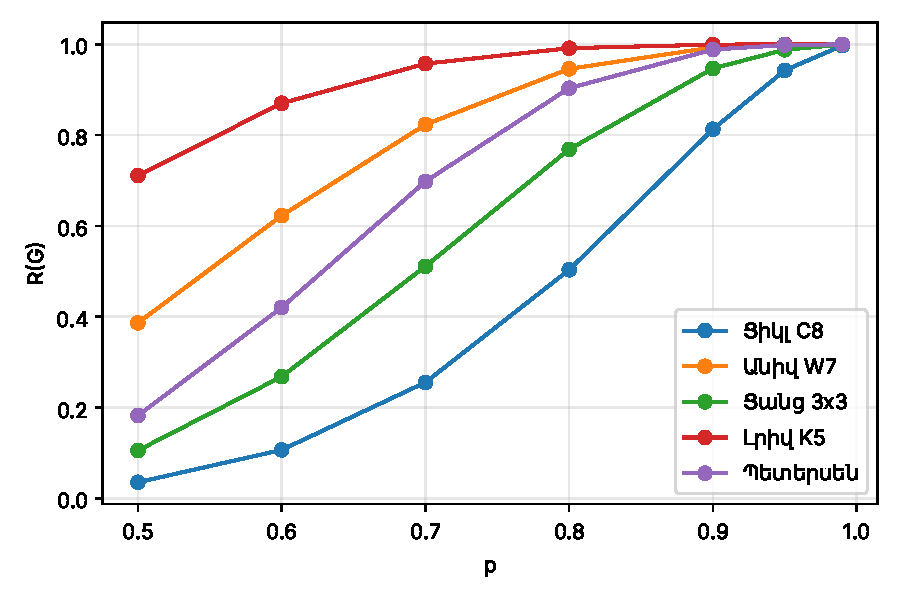
\includegraphics[width=0.8\textwidth]{figures/rel_vs_p.pdf}
\caption{$R(G)$ կախվածությունը կողի աշխատունակության $p$ հավանականությունից}
\end{figure}

\begin{table}[h]
\centering
\small
\begin{tabular}{|l|c|c|c|c|}
\hline
Գրաֆ & $p=0{,}50$ & $p=0{,}80$ & $p=0{,}90$ & $p=0{,}95$\\
\hline
Ցիկլ C8 & 0{,}0352 & 0{,}5033 & 0{,}8131 & 0{,}9428\\
\hline
Անիվ W7 & 0{,}3862 & 0{,}9461 & 0{,}9935 & 0{,}9992\\
\hline
Ցանց 3x3 & 0{,}1052 & 0{,}7688 & 0{,}9470 & 0{,}9882\\
\hline
Լրիվ K5 & 0{,}7109 & 0{,}9917 & 0{,}9995 & 1{,}0000\\
\hline
Պետերսեն & 0{,}1821 & 0{,}9035 & 0{,}9886 & 0{,}9987\\
\hline
\end{tabular}

\caption{Բոլոր գագաթների հուսալիությունը ընտրված $p$ արժեքների համար (ճշգրիտ, գործոնավորմամբ)}
\end{table}

Բոլոր $p$-երի համար գրաֆների դասավորությունը նույնն է. $K_5>W_7>$ Պետերսեն $>3\times3>C_8$: Մեծ $\lambda$-ով գրաֆները ավելի հուսալի են ($K_5$-ի համար $\lambda=4$, $C_8$-ի համար $\lambda=2$), իսկ նույն $\lambda=3$-ի դեպքում ($W_7$ և Պետերսեն) ավելի փոքր գրաֆը ($W_7$, 7 գագաթ) ավելի հուսալի է, որովհետև պետք է կապակցել ավելի քիչ գագաթներ: Տարբերությունը մեծ է. $p=0{,}9$ դեպքում $C_8$-ը կապակցված է մնում ժամանակի $81\%$-ում, իսկ $K_5$-ը՝ $99{,}95\%$-ում:

\subsection{Կապերի ավելացման ազդեցությունը}

Վերցնենք $C_8$ ցիկլը և ավելացնենք 1, ապա 2 լրացուցիչ կող՝ $\{0,4\}$ և $\{2,6\}$:

\begin{table}[h]
\centering
\small
\begin{tabular}{|l|c|c|}
\hline
Գրաֆ & $R$ ($p=0{,}7$) & $R$ ($p=0{,}9$)\\
\hline
C8 & 0{,}2553 & 0{,}8131\\
\hline
C8 + 1 լրաց. կող & 0{,}3739 & 0{,}8896\\
\hline
C8 + 2 լրաց. կող & 0{,}5221 & 0{,}9470\\
\hline
\end{tabular}

\caption{Լրացուցիչ կողերի ազդեցությունը $C_8$ ցիկլի հուսալիության վրա}
\end{table}

Երկու լրացուցիչ կողը $p=0{,}7$ դեպքում հուսալիությունը գրեթե կրկնապատկում է ($0{,}26\to0{,}52$): Հետաքրքիր է, որ $\lambda$-ն այս ընթացքում \emph{չի փոխվում} ($\lambda=2$, քանի որ $1,3,5,7$ գագաթները դեռ ունեն աստիճան 2), թեև հուսալիությունը զգալիորեն աճում է: Սա ցույց է տալիս, որ միայն կապակցվածության թիվը չի բնութագրում ցանցի հուսալիությունը. կարևոր է նաև, թե քանի կտրվածք ունի ցանցը փոքր չափի (տե՛ս բաժին~2.3.3):

\subsection{Կտրվածքային գնահատականներ}

\begin{table}[h]
\centering
\small
\begin{tabular}{|l|c|c|c|}
\hline
Գրաֆ & ստորին & ճշգրիտ $R$ & վերին\\
\hline
Ցիկլ C8 & 0{,}7130 & 0{,}8131 & 0{,}9900\\
\hline
Անիվ W7 & 0{,}9933 & 0{,}9935 & 0{,}9990\\
\hline
Ցանց 3x3 & 0{,}9411 & 0{,}9470 & 0{,}9900\\
\hline
Լրիվ K5 & 0{,}9995 & 0{,}9995 & 0{,}9999\\
\hline
Պետերսեն & 0{,}9880 & 0{,}9886 & 0{,}9990\\
\hline
\end{tabular}

\caption{Թեորեմ~\ref{thm:bounds}-ի գնահատականները, $p=0{,}9$}
\end{table}

Բոլոր դեպքերում ստորին $\le$ ճշգրիտ $\le$ վերին, ինչպես պահանջում է թեորեմը: Ստորին գնահատականը շատ մոտ է ճշգրիտ արժեքին այն գրաֆների համար, որտեղ փոքր կտրվածքները քիչ են ($K_5$, $W_7$, Պետերսեն). տարբերությունը $<0{,}001$: $C_8$-ի համար, որտեղ կան բազմաթիվ 2 կողանի կտրվածքներ, ստորին գնահատականը աղոտ է ($0{,}713$ ընդդեմ $0{,}813$): Վերին գնահատականը (որը օգտագործում է միայն $\lambda$-ն) կոպիտ է, հատկապես փոքր $\lambda$-ի դեպքում:

\subsection{Ճշգրիտ մեթոդներ և Monte Carlo. արագություն և ճշտություն}

Համեմատենք երեք մեթոդները $W_k$ անիվ-գրաֆների վրա ($p=0{,}9$, $m=2(k-1)$ կող). Monte Carlo-ի համար օգտագործվել է $N=20000$ փորձ:

\begin{figure}[h]
\centering
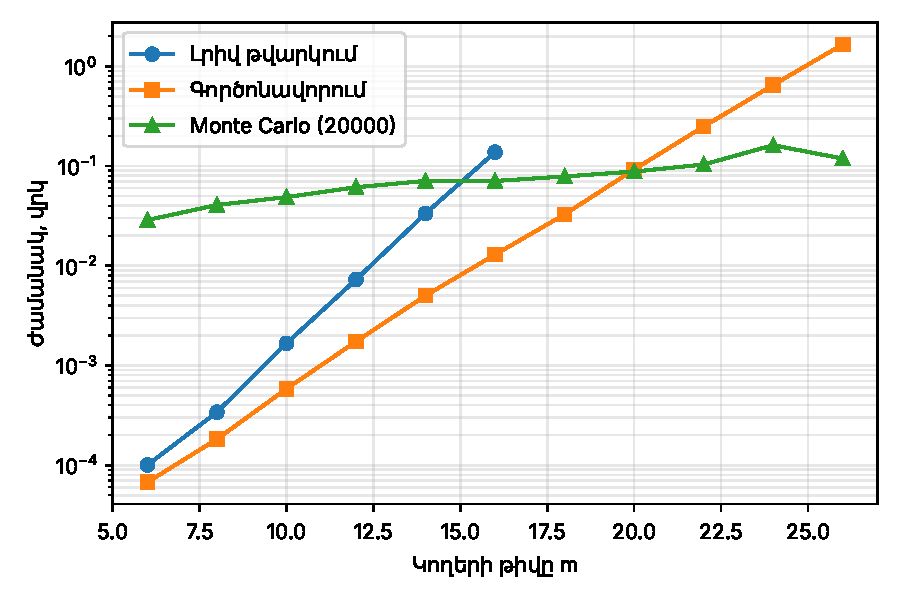
\includegraphics[width=0.8\textwidth]{figures/timing.pdf}
\caption{Մեթոդների աշխատանքի ժամանակը կողերի թվի կախվածությամբ (լոգարիթմական սանդղակ)}
\end{figure}

\begin{table}[h]
\centering
\small
\begin{tabular}{|c|c|c|c|c|c|c|}
\hline
$m$ & թվարկում, վրկ & գործոն., վրկ & MC, վրկ & $R$ ճշգրիտ & $R$ MC & 95\% միջակայք\\
\hline
6 & 0{,}0001 & 0{,}0001 & 0{,}0287 & 0{,}99581 & 0{,}99605 & $\pm$0{,}0009\\
\hline
8 & 0{,}0003 & 0{,}0002 & 0{,}0406 & 0{,}99557 & 0{,}99555 & $\pm$0{,}0009\\
\hline
10 & 0{,}0017 & 0{,}0006 & 0{,}0488 & 0{,}99456 & 0{,}99480 & $\pm$0{,}0010\\
\hline
12 & 0{,}0073 & 0{,}0017 & 0{,}0612 & 0{,}99349 & 0{,}99320 & $\pm$0{,}0011\\
\hline
14 & 0{,}0335 & 0{,}0050 & 0{,}0709 & 0{,}99241 & 0{,}99220 & $\pm$0{,}0012\\
\hline
16 & 0{,}1376 & 0{,}0129 & 0{,}0707 & 0{,}99133 & 0{,}99035 & $\pm$0{,}0014\\
\hline
18 & -- & 0{,}0327 & 0{,}0786 & 0{,}99025 & 0{,}99065 & $\pm$0{,}0013\\
\hline
20 & -- & 0{,}0921 & 0{,}0879 & 0{,}98917 & 0{,}98995 & $\pm$0{,}0014\\
\hline
22 & -- & 0{,}2486 & 0{,}1035 & 0{,}98809 & 0{,}98965 & $\pm$0{,}0014\\
\hline
24 & -- & 0{,}6491 & 0{,}1616 & 0{,}98702 & 0{,}98875 & $\pm$0{,}0015\\
\hline
26 & -- & 1{,}6576 & 0{,}1186 & 0{,}98594 & 0{,}98590 & $\pm$0{,}0016\\
\hline
\end{tabular}

\caption{Ժամանակը և արդյունքը ($p=0{,}9$, $N=20000$). «--»՝ չի չափվել ($m>16$)}
\end{table}

Դիտարկումները.
\begin{itemize}
  \item Լրիվ թվարկումը աճում է մոտավորապես 4 անգամ ամեն 2 նոր կողի համար ($2^2$) և $m=16$ դեպքում արդեն տևում է $\approx0{,}14$ վրկ: Էքստրապոլյացիայով $m=26$ դեպքում դա կլիներ $\approx2$ րոպե, իսկ $m=40$ դեպքում՝ շուրջ մեկ ամիս, ուստի $m>16$ համար թվարկումը չի չափվել:
  \item Գործոնավորումը նույն $m$-երի համար մոտ 10 անգամ արագ է թվարկումից ($m=16$. $0{,}013$ ընդդեմ $0{,}138$ վրկ) շնորհիվ վաղ էտման, բայց նրա ժամանակն էլ է աճում էքսպոնենցիալ ($m=26$. $\approx1{,}7$ վրկ):
  \item Monte Carlo-ի ժամանակը աճում է մոտավորապես գծային ($0{,}03\to0{,}12$ վրկ $m=6\to26$ դեպքում, չափումները աղմկոտ են): Գործոնավորման և Monte Carlo-ի ժամանակները հավասարվում են $m\approx20$ դեպքում ($\approx0{,}09$ վրկ երկուսի համար). $m=22$ դեպքում գործոնավորումը $0{,}25$ ընդդեմ $0{,}10$ վրկ է, իսկ $m=26$ դեպքում՝ $\approx14$ անգամ դանդաղ:
  \item Monte Carlo-ի 95\% միջակայքը ($\approx\pm0{,}001$--$0{,}0016$) պարունակել է ճշգրիտ արժեքը 11 դեպքից 9
-ում: Մնացած դեպքերում շեղումը մի փոքր գերազանցել է միջակայքը (մինչև $1{,}2$ անգամ). նկատենք, որ բոլոր չափումների համար օգտագործվել է նույն սերմը (\texttt{seed=3}), ուստի սխալները միմյանցից անկախ չեն:
\end{itemize}

\subsection{Monte Carlo-ի սխալի կախումը փորձերի թվից}

$3\times3$ ցանցի համար ($p=0{,}8$, ճշգրիտ $R=0{,}7688$) $N$-ի տարբեր արժեքներով 10 անկախ սերմերով հաշվվել է միջին բացարձակ սխալը:

\begin{figure}[h]
\centering
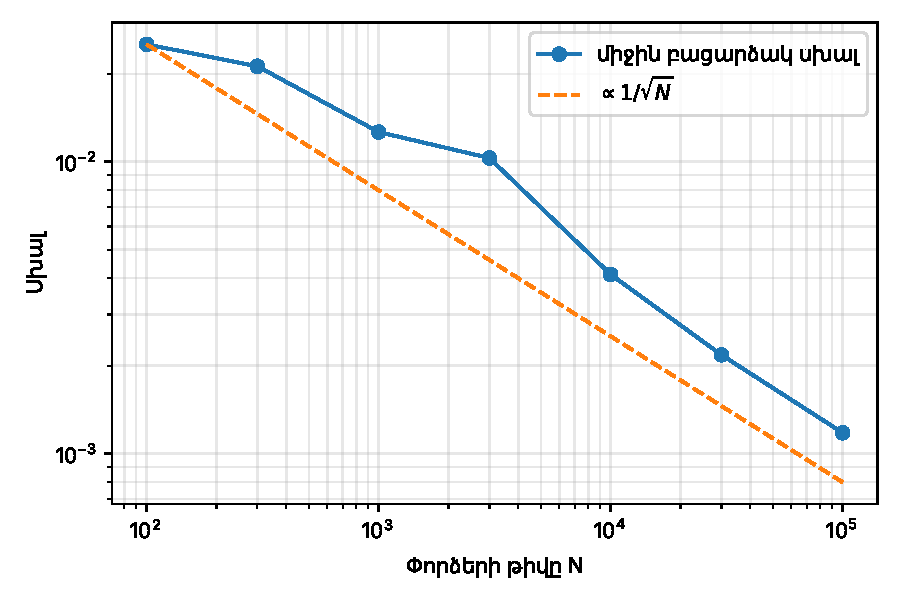
\includegraphics[width=0.8\textwidth]{figures/mc_error.pdf}
\caption{Monte Carlo-ի սխալը՝ ըստ $N$-ի (լոգարիթմական սանդղակ), կետագիծը՝ $1/\sqrt N$ կախվածությունը}
\end{figure}

\begin{table}[h]
\centering
\small
\begin{tabular}{|r|c|}
\hline
$N$ & միջին $|\widehat R_N-R|$\\
\hline
100 & 0{,}02524\\
\hline
300 & 0{,}02124\\
\hline
1000 & 0{,}01264\\
\hline
3000 & 0{,}01030\\
\hline
10000 & 0{,}00411\\
\hline
30000 & 0{,}00218\\
\hline
100000 & 0{,}00118\\
\hline
\end{tabular}

\caption{Monte Carlo-ի միջին բացարձակ սխալը}
\end{table}

$N$-ը 1000 անգամ մեծացնելիս ($100\to10^5$) սխալը փոքրացել է մոտ 21 անգամ, ինչը մոտ է տեսականին՝ $\sqrt{1000}\approx32$ (միջինացումը ընդամենը 10 սերմի վրա է, այդ պատճառով կորը աղմկոտ է): Եզրակացությունը համապատասխանում է Բաժին~2.4-ի. սխալը նվազում է $1/\sqrt N$ արագությամբ:

\section{Ամփոփում}

Փորձերը հաստատում են տեսական եզրակացությունները.
\begin{enumerate}
  \item ճշգրիտ մեթոդները (թվարկում, գործոնավորում) տալիս են նույն արդյունքը և կիրառելի են $m\lesssim25$ կողի համար, դրանից հետո ժամանակը աճում է էքսպոնենցիալ.
  \item Monte Carlo-ն ունի գծային բարդություն և հնարավորություն է տալիս գնահատել մեծ գրաֆները, սակայն ճշտությունը լավացնելու գինը $N\propto1/\varepsilon^2$ է.
  \item կապակցվածության չափանիշները ($\lambda$, $\kappa$) և հուսալիությունը կապված են, բայց հուսալիությունը կախված է նաև կտրվածքների թվից (օրինակ՝ լրացուցիչ կող ավելացնելը $\lambda$-ն չփոխելով բարձրացնում է $R$-ը).
  \item կտրվածքային գնահատականները շատ ճշգրիտ են բարձր $p$-ի և քիչ փոքր կտրվածքներով գրաֆների համար:
\end{enumerate}

\textbf{Սահմանափակումներ.} Փորձարկումը կատարվել է փոքր մոդելային գրաֆների վրա, բոլոր կողերը ունեն նույն $p$ և գագաթները չեն խափանվում: Իրական ցանցերի (օրինակ՝ մայրուղային կամ հաղորդակցական ցանցերի տոպոլոգիաներ) վրա փորձարկումը և գագաթային խափանումների մոդելը կարող են ավելացվել հետագա աշխատանքում:


\chapter*{Եզրակացություն}
\addcontentsline{toc}{chapter}{Եզրակացություն}

% Սևագիր v1: կճշգրտվի Գլուխ 1-3-ը վերջնականապես հաստատելուց հետո
Աշխատանքում ուսումնասիրվել են գրաֆների կապակցվածության և ցանցի հուսալիության վերլուծության հիմնական մեթոդները: Ներկայացվել են կապակցվածության հասկացությունները (կամուրջներ, կտրող կետեր, $k$-կապակցվածություն, Մենգերի թեորեմ), կապակցվածության որոշման և չափման ալգորիթմները (BFS/DFS, Տարյանի ալգորիթմ, առավելագույն հոսք), հուսալիության ճշգրիտ (թվարկում, գործոնավորում) և մոտավոր (Monte Carlo) մեթոդները, ինչպես նաև կտրվածքային գնահատականները: Բոլոր ալգորիթմները իրականացված են Python լեզվով, ստուգված են \texttt{NetworkX}-ի հետ համեմատությամբ և փորձարկված են 5 մոդելային գրաֆների վրա: Փորձերը ցույց են տվել, որ ճշգրիտ մեթոդները կիրառելի են մինչև մոտ 25 կող ունեցող գրաֆների համար, Monte Carlo-ն թույլ է տալիս գնահատել ավելի մեծ գրաֆներ $1/\sqrt N$ ճշտությամբ, իսկ հուսալիությունը կախված է ոչ միայն $\lambda$-ից, այլև փոքր կտրվածքների քանակից.

\clearpage
\addcontentsline{toc}{chapter}{Գրականության ցանկ}
\begin{thebibliography}{9}
\bibitem{west} D.~B.~West, \emph{Introduction to Graph Theory}, Prentice Hall, 2001.
\bibitem{colbourn} C.~J.~Colbourn, \emph{The Combinatorics of Network Reliability}, Oxford University Press, 1987.
\bibitem{valiant} L.~G.~Valiant, The complexity of enumeration and reliability problems, \emph{SIAM J. Computing}, 8(3), 1979, 410--421.
\bibitem{tarjan} R.~E.~Tarjan, Depth-first search and linear graph algorithms, \emph{SIAM J. Computing}, 1(2), 1972, 146--160.
\bibitem{edmondskarp} J.~Edmonds, R.~M.~Karp, Theoretical improvements in algorithmic efficiency for network flow problems, \emph{J. ACM}, 19(2), 1972, 248--264.
\bibitem{provanball} J.~S.~Provan, M.~O.~Ball, The complexity of counting cuts and of computing the probability that a graph is connected, \emph{SIAM J. Computing}, 12(4), 1983, 777--788.
\bibitem{metropolis} N.~Metropolis, S.~Ulam, The Monte Carlo method, \emph{J. Amer. Statist. Assoc.}, 44(247), 1949, 335--341.
\end{thebibliography}

\end{document}
